\documentclass[notes,serif]{beamer}
\usepackage{graphicx}
\usepackage{url}
\usepackage{clrscode}
\usepackage{amssymb,amsmath}

% You should run 'pdflatex' TWICE, because of TOC issues.

\mode<presentation>
{
  % A tip: pick a theme you like first, and THEN modify the color theme, and then add math content.
  % Warsaw is the theme selected by default in Beamer's installation sample files.

  %%%%%%%%%%%%%%%%%%%%%%%%%%%% THEME
  %\usetheme{AnnArbor}
  %\usetheme{Antibes}
  %\usetheme{Bergen}
  %\usetheme{Berkeley}
  %\usetheme{Berlin}
  %\usetheme{Boadilla}
  %\usetheme{boxes}
  %\usetheme{CambridgeUS}
  %\usetheme{Copenhagen}
  %\usetheme{Darmstadt}
  %\usetheme{default}
  %\usetheme{Dresden}
  %\usetheme{Frankfurt}
  %\usetheme{Goettingen}
  %\usetheme{Hannover}
  %\usetheme{Ilmenau}
  %\usetheme{JuanLesPins}
  %\usetheme{Luebeck}
  %\usetheme{Madrid}
  %\usetheme{Malmoe}
  %\usetheme{Marburg}
  %\usetheme{Montpellier}
  %\usetheme{PaloAlto}
  %\usetheme{Pittsburgh}
  %\usetheme{Rochester}
  %\usetheme{Singapore}
  %\usetheme{Szeged}
  \usetheme{Warsaw}

  %%%%%%%%%%%%%%%%%%%%%%%%%%%% COLOR THEME
  %\usecolortheme{albatross}
  %\usecolortheme{beetle}
  %\usecolortheme{crane}
  \usecolortheme{default}
  %\usecolortheme{dolphin}
  %\usecolortheme{dove}
  %\usecolortheme{fly}
  %\usecolortheme{lily}
  %\usecolortheme{orchid}
  %\usecolortheme{rose}
  %\usecolortheme{seagull}
  %\usecolortheme{seahorse}
  %\usecolortheme{sidebartab}
  %\usecolortheme{structure}
  %\usecolortheme{whale}

  %%%%%%%%%%%%%%%%%%%%%%%%%%%% OUTER THEME
  %\useoutertheme{default}
  %\useoutertheme{infolines}
  %\useoutertheme{miniframes}
  %\useoutertheme{shadow}
  %\useoutertheme{sidebar}
  %\useoutertheme{smoothbars}
  %\useoutertheme{smoothtree}
  %\useoutertheme{split}
  %\useoutertheme{tree}

  %%%%%%%%%%%%%%%%%%%%%%%%%%%% INNER THEME
  %\useinnertheme{circles}
  %\useinnertheme{default}
  %\useinnertheme{inmargin}
  %\useinnertheme{rectangles}
  %\useinnertheme{rounded}

  %%%%%%%%%%%%%%%%%%%%%%%%%%%%%%%%%%%

%  \setbeamercovered{transparent} % or whatever (possibly just delete it)
  \setbeamercovered{invisible} % or whatever (possibly just delete it)
  % To change behavior of \uncover from graying out to totally invisible, can change \setbeamercovered to invisible instead of transparent. apparently there are also 'dynamic' modes that make the amount of graying depend on how long it'll take until the thing is uncovered.

}


% Get rid of nav bar
\beamertemplatenavigationsymbolsempty

% Use short top
%\usepackage[headheight=12pt,footheight=12pt]{beamerthemeboxes}
%\addheadboxtemplate{\color{black}}{
%\hskip0.3cm
%\color{white}
%\insertshortauthor \ \ \ \
%\insertframenumber \ \ \ \ \ \ \
%\insertsection \ \ \ \ \ \ \ \ \ \ \ \ \ \ \ \ \  \insertsubsection
%\hskip0.3cm}
%\addheadboxtemplate{\color{black}}{
%\color{white}
%\ \ \ \
%\insertsection
%}
%\addheadboxtemplate{\color{black}}{
%\color{white}
%\ \ \ \
%\insertsubsection
%}

% Insert frame number at bottom of the page.
\usefoottemplate{\hfil\tiny{\color{black!90}\insertframenumber}}

\usepackage[english]{babel}
\usepackage[latin1]{inputenc}

\usepackage{times}
\usepackage[T1]{fontenc}

\title{Network Programming}
\subtitle{Lecture 2---Elementary Sockets I}

\author{Lei Wang\\ lei.wang@dlut.edu.cn}

\institute{Dalian University of Technology}

%\date{Date}
\date{Nov 24, 2008}

\subject{Talks}

\def\defn#1{{\color{red} #1}}

\begin{document}

\begin{frame}
  \titlepage
\end{frame}

\begin{frame}
  \frametitle{Part 2. Elementary Sockets I}
  \tableofcontents
\end{frame}

\section{Sockets Introduction}
\subsection{Socket Address Structures}

\begin{frame}[containsverbatim]
\frametitle{Socket Address Structures}
%
\begin{itemize}
  \item Most socket functions require a pointer to a socket address structure as an
argument.
  \item Each supported protocol suite defines its own socket address structure.
  \item The names of these structures begin with \texttt{sockaddr\_} and end with a unique suffix
for each protocol suite.
\end{itemize}
\end{frame}

\begin{frame}[containsverbatim]
\frametitle{IPv4 Socket Address Structure}
  \begin{figure}
  \centering
  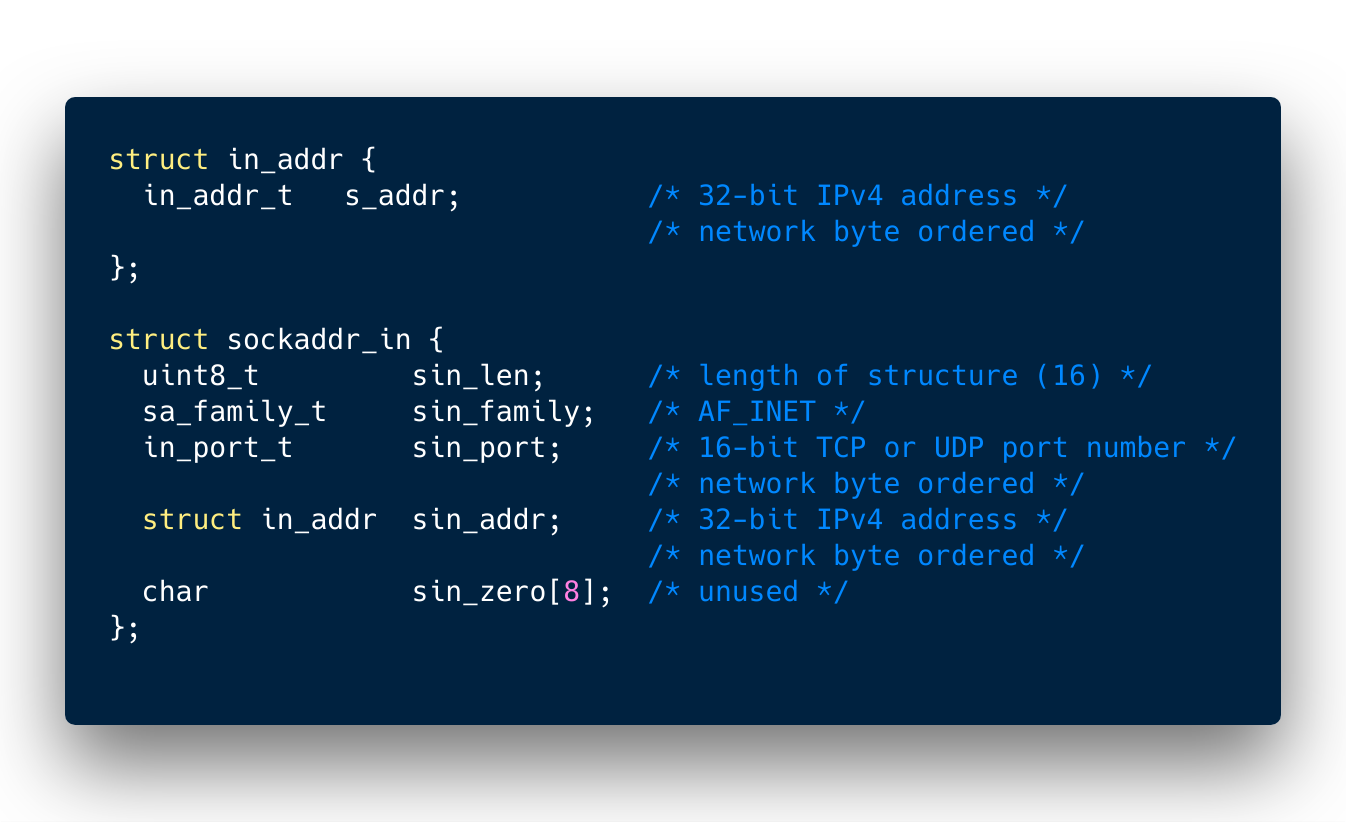
\includegraphics[width=.8\textwidth]{code/02code01.png}\\
  \caption{IPV4 socket address structure}
  \label{1}
  \end{figure}
\end{frame}


\begin{frame}[containsverbatim]
\frametitle{Generic Address Structure}
  \begin{figure}
  \centering
  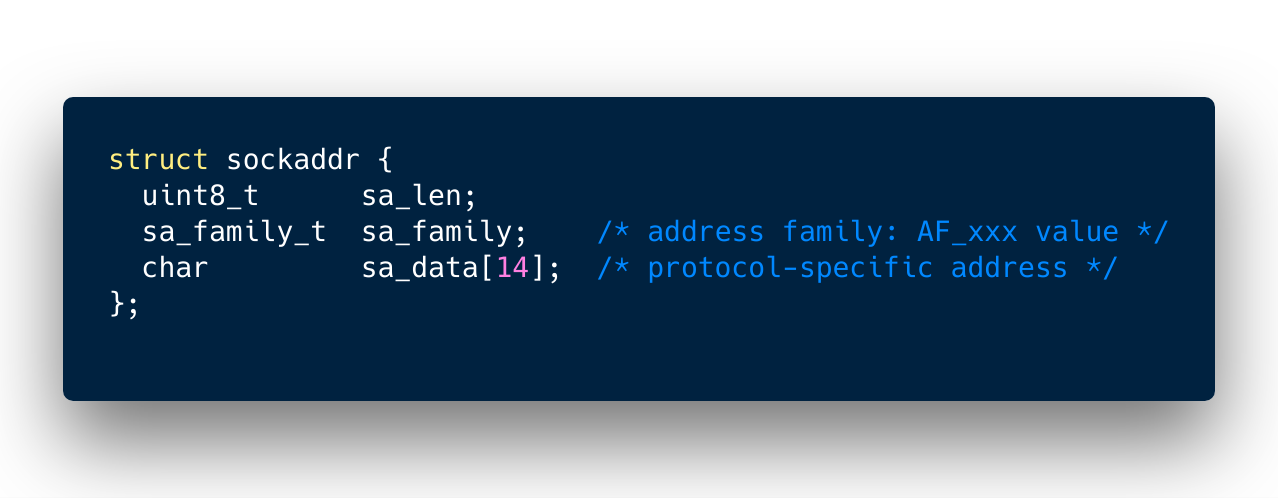
\includegraphics[width=.8\textwidth]{code/02code02.png}\\
  \caption{Generic Address Structure}
  \label{2}
  \end{figure}
\end{frame}


\begin{frame}[containsverbatim]
\frametitle{IPv6 Socket Address Structure}
  \begin{figure}
  \centering
  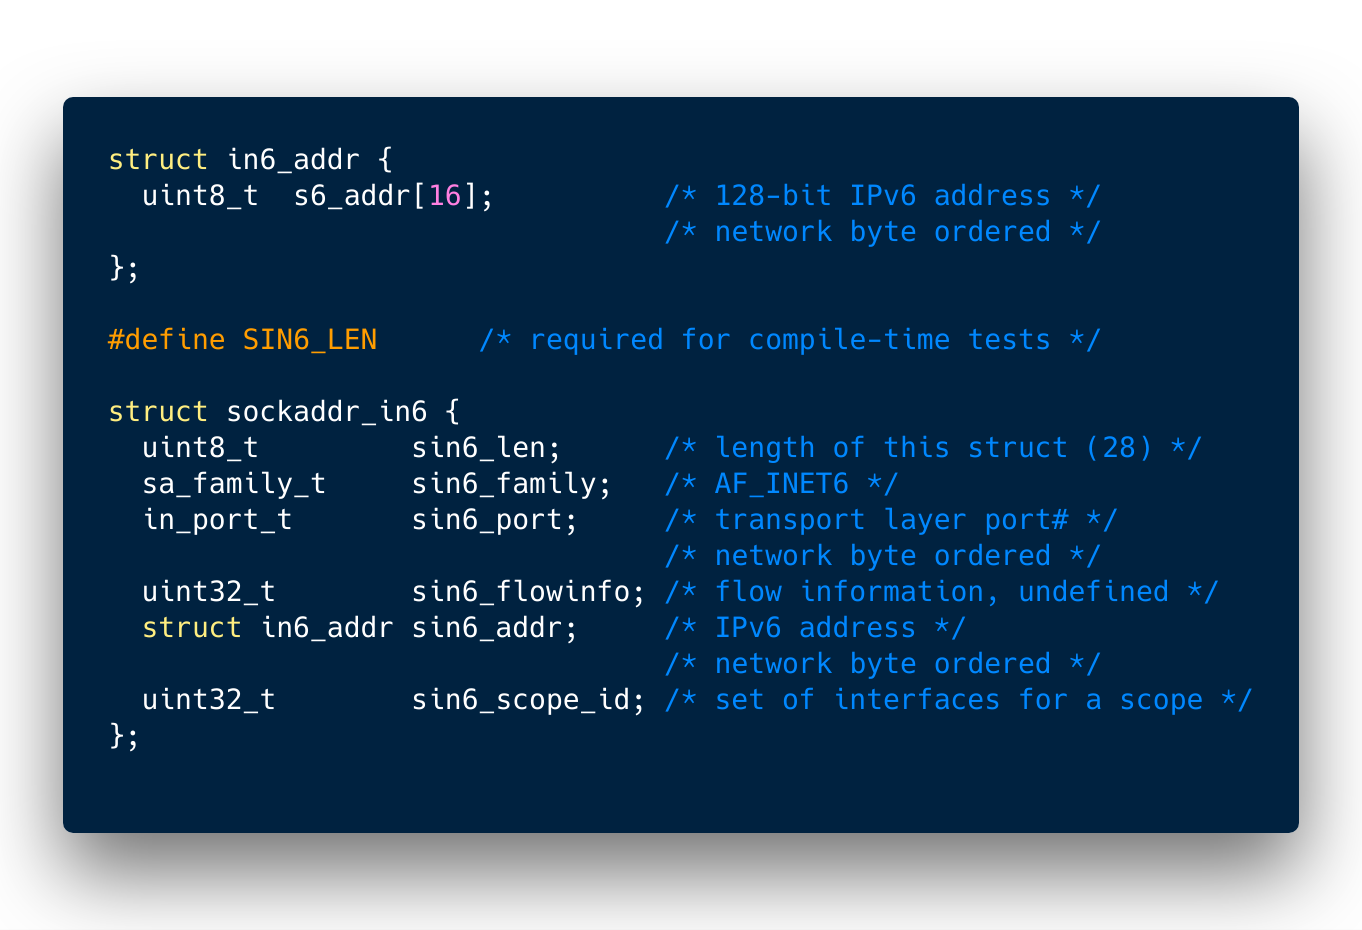
\includegraphics[width=.8\textwidth]{code/02code03.png}\\
  \caption{IPv6 Socket Address Structure}
  \label{3}
  \end{figure}
\end{frame}

\subsection{Value-Result Arguments}

\begin{frame}[containsverbatim]
\frametitle{Value-Result Arguments}
  %% \begin{center}
  %% 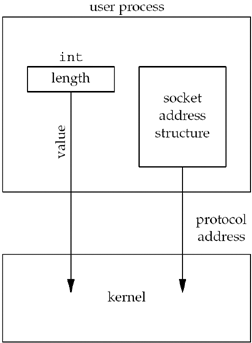
\includegraphics[width=.4\textwidth]{figs/03fig07.png}
  %% \vspace{4em}
  %% 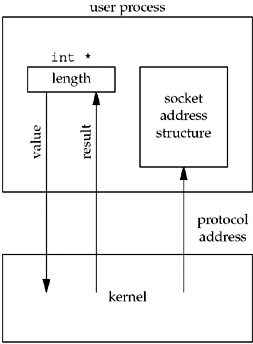
\includegraphics[width=.4\textwidth]{figs/03fig08.png}
  %% \end{center}
  \begin{figure}
    \centering
    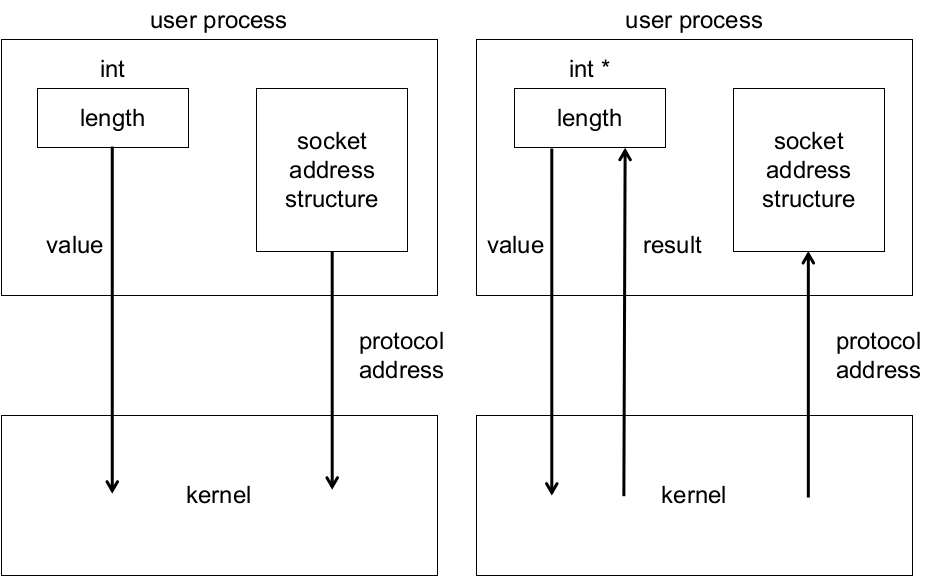
\includegraphics[width=.8\textwidth]{fig/02fig01.png}
  \end{figure}
\end{frame}

\subsection{Byte Ordering}
\begin{frame}
\frametitle{Byte Ordering}
  \begin{center}
  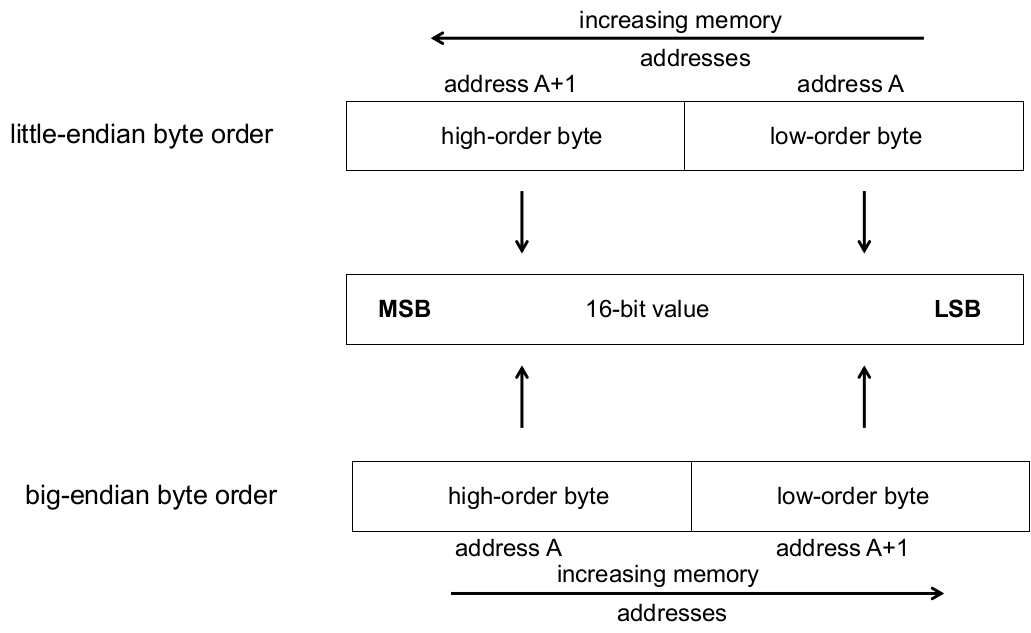
\includegraphics[width=.8\textwidth]{fig/02fig02.png}
  \end{center}
\end{frame}

\begin{frame}[containsverbatim]
\frametitle{\texttt{byteorder.c}} 
  \begin{figure}
  \centering
  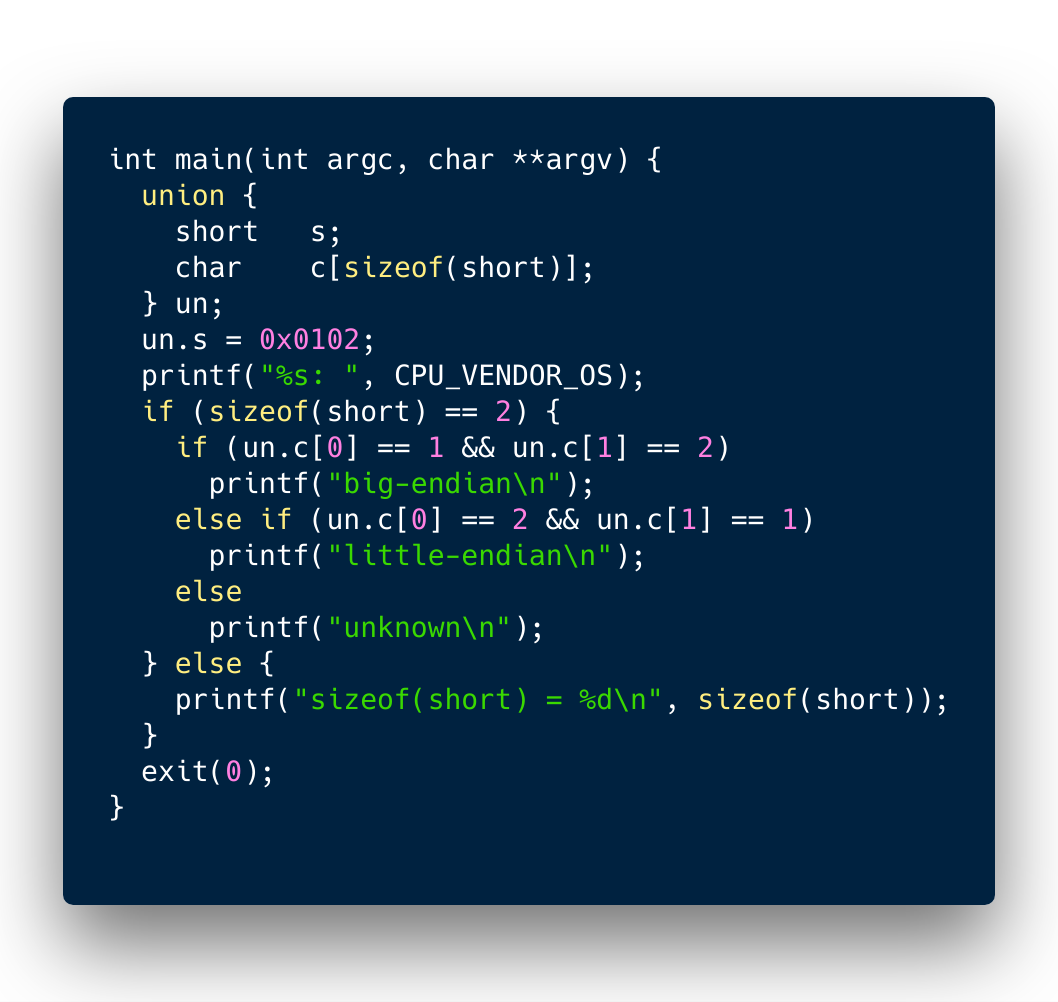
\includegraphics[width=.7\textwidth]{code/02code04.png}\\
  \caption{byteorder.c}
  \label{4}
  \end{figure}
\end{frame}

\section{Elementary TCP Sockets}

\subsection{Elementary Sockets Functions}
\subsubsection{\texttt{socket, connect, bind, listen, accept}}
\begin{frame}
  \frametitle{Elementary Sockets Functions}
  \begin{itemize}
    \item \texttt{socket}
    \item \texttt{connect}
    \item \texttt{bind}
    \item \texttt{listen}
    \item \texttt{accept}
  \end{itemize}
\end{frame}

%\begin{frame}
%  \frametitle{{\bf \texttt{socket(...)}}}
%  % the prototype of socket()
%\end{frame}

\subsection{Concurrent Servers}
\begin{frame}[containsverbatim]
  \frametitle{Concurrent Servers}
  \begin{figure}
  \centering
  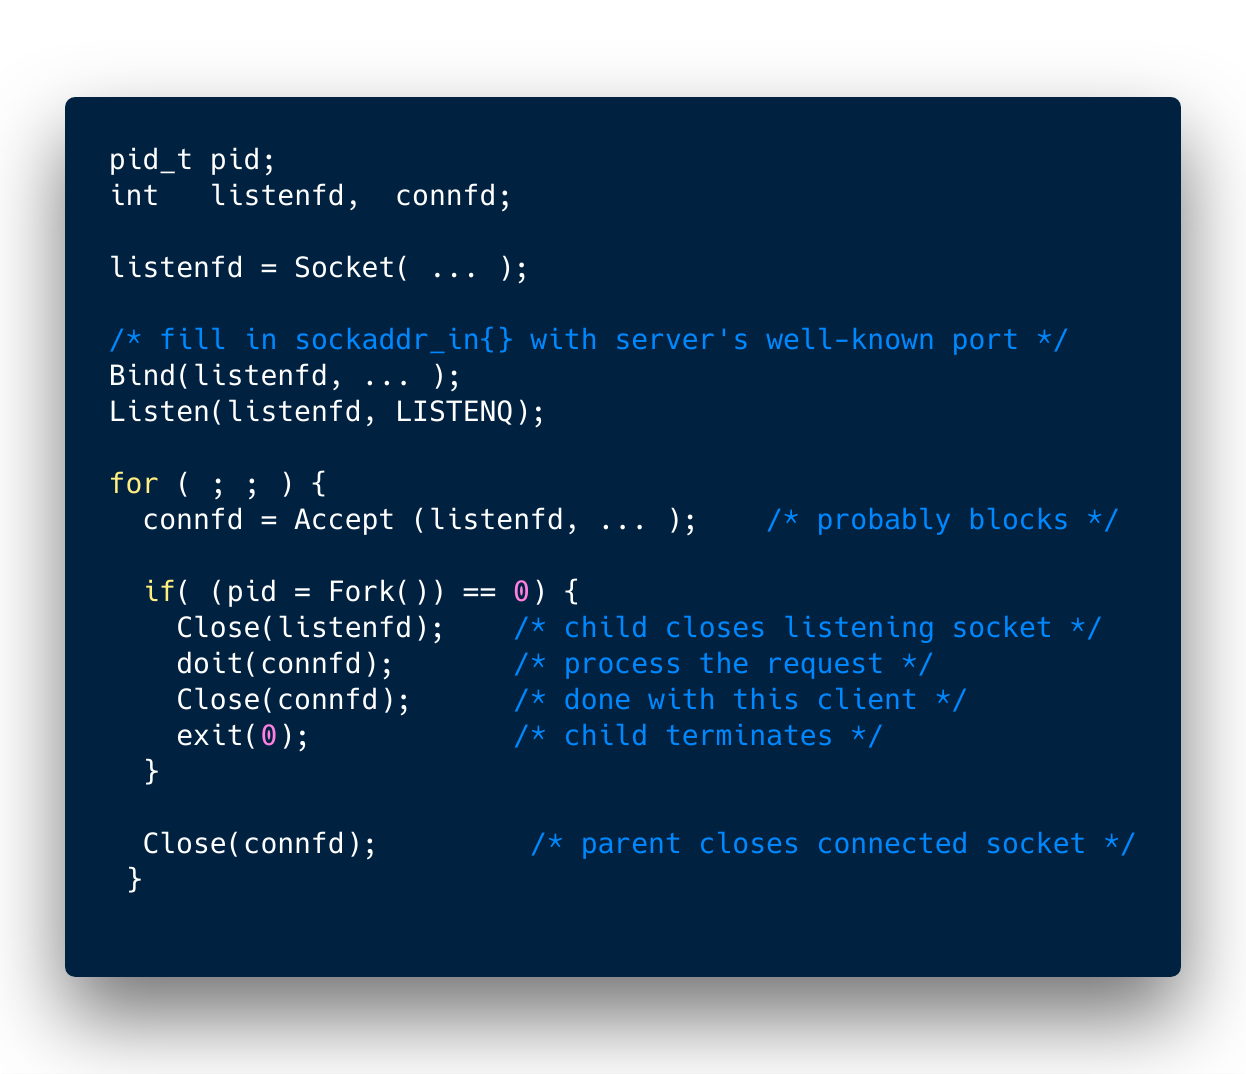
\includegraphics[width=.7\textwidth]{code/02code05.png}\\
  \caption{Concurrent Servers}
  \label{5}
  \end{figure}
\end{frame}

\subsection{\texttt{close} Function}
\begin{frame}
  \frametitle{\texttt{close} Function}
  \begin{itemize}
    \item Descriptor Reference Counts
    \item {\tt shutdown} for mandatory FIN
  \end{itemize}
\end{frame}

%\subsection{\texttt{getsockname \text{and} getpeername} Functions}
%\begin{frame}
%  \frametitle{\texttt{getsockname \text{and} getpeername} Functions}
%\end{frame}

\section{TCP Client/Server Example}
\begin{frame}
  \frametitle{TCP Client/Server Example}
\begin{itemize}
  \item TCP Echo Client/Server
  \item Chapter 5---homework and experiment assignment  %(��ҵ���ϻ�)
\end{itemize}
\end{frame}

\subsection{Summary}
\begin{frame}
  \frametitle{Summary}
  \begin{itemize}
    \item All clients and servers call to \texttt{socket}, returning a socket descriptor.
    \item Clients then call \texttt{connect}, while servers call \texttt{bind}, \texttt{listen}, and \texttt{accept}.
    \item Sockets are normally closed with the standard close function, although another way is the \texttt{shutdown}
    function.
  \end{itemize}
\end{frame}

\end{document}
